\section{Evaluation}
\label{eval}
%Evaluation section...
%
%Length: 3-4 pages (graphs take a lot of space!)
%
%Tell reader what to expect.
%
%Eval is "proof" that your design is good.
%MATCH eval goals with design goals.
%
%Eval section is easier to write, but longest one to produce
%results for.  Whereas design section has complex structure, eval
%is more 'flat'.
%
%Structure:
%
%1.  list eval goals, should match design goals
%
%2.  briefly list how you plan to prove those goals.
%
%3.  describe your testbed: h/w + s/w platform to run tests on.
%Give enough detail so it can be reproduced by ANYONE.
%
%4.  describe your benchmarks in detail:
%
%(4a) Micro benchmarks: test specific feature (e.g., read or
%write performance).  Usually u-bench are designed to highlight
%worst/best case behavior of your system.  Be to list both best
%and worst.
%
%(4b) Macro benchmarks (general purpose benchmarks): test whole
%system (e.g., run a Web server exerciser, or TPC for database).
%
%Some tests should compare YOUR system to past systems, or a
%"before and after" comparison.
%
%For every possible variable in your system, design a set of
%independent tests (re: compression study's dimensions).  Justify
%need to vary each variable (the more variables, the more
%experiments you have to run).
%
%5.  Describe your benchmarking methodology
%
%Statistical stability: how many times you run each test? do you
%compute standard deviations, half-width intervals (for student-t
%distribution), RMS, or other metric of stability?  Say how many
%times you ran each test, and what were the stability metrics.
%
%Ex."we ran every test at least 10 times, and computed the
%standard deviation as a percentage of the mean.  In all cases,
%the percentage was less than 5\%, unless otherwise noted."
%
%6.  List every benchmark result, for each test
%
%(a) a graph or table or other figure, plus caption.
%(b) followed by an explanation of the figure: say what one sees
%    in the figure, then explain WHY it is so.
%
%7.  Optional: if eval section longer than usual, end it with a
%one-paragraph summary of eval results.

\paragraph{Evaluation Goals} The project aimed to perform a thorough
benchmarking of existing BFS algorithms for energy efficiency and
related parameters. This broader goal was further sub-categorized into
following:
\begin{itemize}
\item
\textbf{Exploration \& Collection of existing BFS implementations}\\
We successfully explored existing literature on BFS, collected
\emph{six} BFS implementations, brought them into runnable state and
verified their correctness.
\item
\textbf{Collecting Dataset \& Coverting it into appropriate format}\\
We collected \emph{eleven} graph datasets from \emph{Florida Sparse
Matrix} ~\cite{FLORIDA-SPARSE} database and pre-processed them to a
form accepted by the algorithm.
\item
\textbf{Benchmarking of the Algorithms based on various parameters}\\
For this purpose we used environment, tools and settings described
previously in the design section.
\end{itemize}

\paragraph{Results, Observations \& Analysis}
Results can divided into following sets:
\begin{itemize}
\item
\textbf{Runtime Results}
Table \ref{tab:RuntimeTable} shows the running time for the six
algorithms.  Visual representation for same is shown in \emph{Figure
1}.  As can be observed, though Algorithm 6 performed better for
smaller datasets, Algorithm 4 out-passed it and other algorithms in
terms of runtime for larger datasets.  This can be due to the reason
that the algorithm tries to exploit maximum parallelism and avoids
revisiting of the edges which reduces the overall work significantly.
\begin{figure}[t]
    \centering
    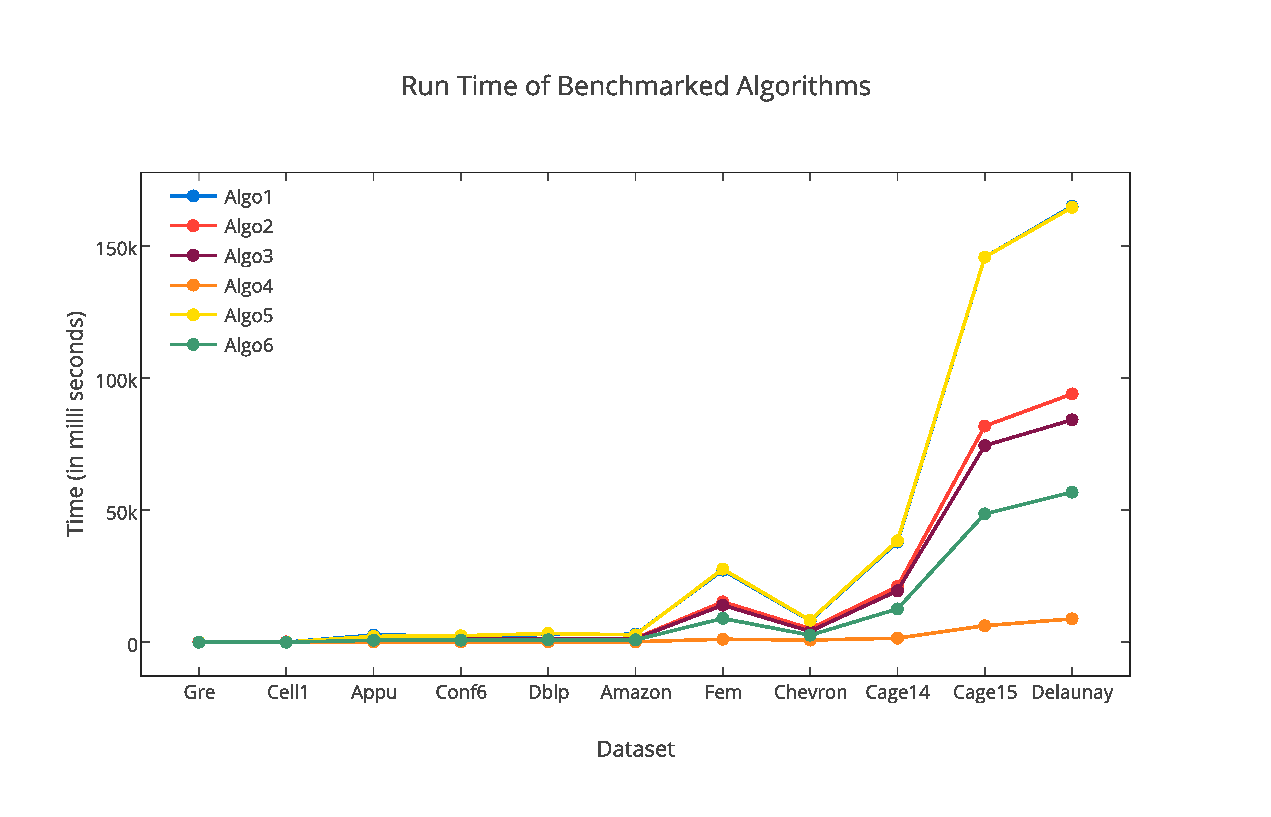
\includegraphics[width=0.5\textwidth]{figures/RunTimeofBenchmarkedAlgorithms.eps}
    \caption{Run Time (in ms)}
    \label{fig:Run Time}
\end{figure}
\begin{table*}[th]
\begin{center}
    \begin{tabular}{| l | l | l | l | l | l | l |}
    \hline
	Dataset & Algo1 & Algo2 & Algo3 & Algo4 & Algo5 & Algo6\\ \hline
    \hline
	Gre & 11.276 & 89.645 & 9.35 & 14.90 & 14.23 & \cellcolor{blue!25} 2.84\\ \hline
	Cell1 & 57.456 & 169.51 & 23.15 & 53.67 & 56.20 & \cellcolor{blue!25} 19.36\\ \hline
	Appu & 2729.78 & 1277.10 & 1230.77 & \cellcolor{blue!25} 127.39 & 2226.78 & 753.26\\ \hline
	Conf6 & 2456.12 & 1373.91 & 1312.49 & \cellcolor{blue!25} 123.89 & 2471.88 & 795.07\\ \hline
	Dblp & 2927.43 & 1671.65 & 1485.92 & \cellcolor{blue!25} 170.13 & 3316.42 & 948.97\\ \hline
	Amazon & 3022.22 & 1478.76 & 1336.50 & \cellcolor{blue!25} 206.07 & 2793.10 & 926.2\\ \hline
	Fem & 27272.80 & 15298.61 & 14042.00 & \cellcolor{blue!25} 1153.52 & 27702.53 & 9024.60\\ \hline
	Chevron & 8155.47 & 5139.08 & 4140.09 & \cellcolor{blue!25} 832.14 & 8318.43 & 2675.63\\ \hline
	Cage14 & 37933.25 & 21091.25 & 19476.28 & \cellcolor{blue!25} 1548.31 & 38384.06 & 12608.33\\ \hline
	Cage15 & 145707.52 & 81805.62 & 74409.52 & \cellcolor{blue!25} 6254.28 & 145729.76 & 48580.77\\ \hline
	Delaunay & 165012.42 & 93963.65 & 84164.53 & \cellcolor{blue!25} 8868.07 & 164585.42 & 56794.18\\ \hline
    \end{tabular}
\end{center}
\caption{\capfont Running time (in ms)}
\label{tab:RuntimeTable}
\end{table*}
\item
\textbf{L2CACHE, L3CACHE Performance Results}
\begin{table*}[th]
\small
\centering
%\begin{tabularx}{\linewidth}{|c|c|c|c|c|c|c|X|}

\begin{tabular}{ c|c|c|c|c|c|c|c|c|c|c|c|c| }
%  \cline{2-13}
\hline
\multicolumn{1}{|c|}{\textbf{Dataset}} &
\multicolumn{6}{c}{\textbf{L2CACHE}} &
  \multicolumn{6}{|c|}{\textbf{L3CACHE}} \\
  \cline{2-13}
  \multicolumn{1}{|c|}{} &
  Algo1 & Algo2 & Algo3 & Algo4 & Algo5 & Algo6 & Algo1 & Algo2 & Algo3 & Algo4 & Algo5 & Algo6\\\hline
    \hline
  \multicolumn{1}{|c|}{\textbf{Gre}}
& 4.55 & 4.03 & 4.81 & \cellcolor{blue!25}3.45 & 3.57 & 3.85 & 4.66 & 5.07 & \cellcolor{green!25}4.06 & 7.46 & 5.12 & 4.96 \\ \hline
  \multicolumn{1}{|c|}{\textbf{Cell1}}
& 4.69 & 3.73 & \cellcolor{blue!25}3.66 & 4.98 & 4.78 & 4.17 & 6.12 & 4.67 & \cellcolor{green!25}4.02 & 13.97 & 7.66 & 7.67\\ \hline
  \multicolumn{1}{|c|}{\textbf{Appu}}
& 3.54 & 5.10 & 3.84 & \cellcolor{blue!25}3.49 & 4.31 & 4.54 & \cellcolor{green!25}4.51 & 4.61 & 7.73 & 10.13 & 5.38 & 5.29\\ \hline
\multicolumn{1}{|c|}{\textbf{Conf6}}
& 4.99 & 4.14 & 4.67 & \cellcolor{blue!25}3.81 & 5.07 & 4.49 & \cellcolor{green!25}5.16 & 5.77 & 8.58 & 10.94 & 5.57 & 5.47\\ \hline
  \multicolumn{1}{|c|}{\textbf{Dblp}}
& 4.68 & 4.25 & 5.11 & \cellcolor{blue!25}3.92 & 5.03 & 4.65 & \cellcolor{green!25}4.77 & 9.65 & 9.34 & 11.30 & 7.18 & 7.18\\ \hline
  \multicolumn{1}{|c|}{\textbf{Amazon}}
& 4.70 & 4.39 & 5.07 & \cellcolor{blue!25}3.35 & 4.98 & 4.54 & \cellcolor{green!25}5.40 & 10.80 & 13.02 & 9.34 & 8.38 & 8.65\\ \hline
  \multicolumn{1}{|c|}{\textbf{Fem}}
& 4.83 & 4.15 & 4.62 & \cellcolor{blue!25}3.97 & 4.92 & 4.67 & 5.21 & 9.07 & 9.49 & 10.11 & \cellcolor{green!25}5.15 & 6.84\\ \hline
  \multicolumn{1}{|c|}{\textbf{Chevron4}}
& 4.85 & 4.10 & 4.70 & \cellcolor{blue!25}4.09 & 5.04 & 4.50 & 8.62 & \cellcolor{green!25}4.21 & 10.85 & 13.68 & 11.46 & 12.02\\ \hline
  \multicolumn{1}{|c|}{\textbf{Cage14}}
& 4.76 & \cellcolor{blue!25}4.03 & 4.97 & 4.03 & 4.92 & 4.59 & \cellcolor{green!25}4.86 & 9.15 & 10.46 & 9.58 & 5.18 & 5.77\\ \hline
  \multicolumn{1}{|c|}{\textbf{Cage15}}
& 4.61 & 4.09 & 4.83 & \cellcolor{blue!25}3.84 & 4.56 & 4.75 & \cellcolor{green!25}5.28 & 10.12 & 7.94 & 9.65 & 5.31 & 5.46\\ \hline
  \multicolumn{1}{|c|}{\textbf{Delaunay}}
& 4.36 & 4.08 & 4.69 & \cellcolor{blue!25}4.06 & 4.34 & 4.61 & \cellcolor{green!25}5.84 & 16.00 & 7.63 & 6.54 & 7.63 & 8.18\\ \hline
\end{tabular}

%\end{tabularx}
\caption{\capfont L2CACHE and L3CACHE miss ratio readings }
\label{tab:Table6}
\end{table*}
From Table~\ref{tab:Table6} we can see that Algorithm 4 performs best
for most of the times in L2CACHE measure.  This algorithm is observed
to be makinng best use of the system hardware which might be affecting
its L2CACHE performance.
\newline
From Table~\ref{tab:Table6} we can see that
Algorithm 1's L3CACHE performance is best for most of the times.  A
work-stealing technique steals from neighbouring threads running on
the same socket which improves cache efficiency. Also the algorithm is
lock-free and so cache flush in cases of lock conflicts is not
present.
\begin{figure}[t]
    \centering
    \includegraphics[width=0.5\textwidth]{figures/CacheMissRatioforAppu.eps}
    \caption{Cache-miss ratio for Appu}
    \label{fig:Appu-Cache Miss}
\end{figure}

\begin{figure}[t]
    \centering
    \includegraphics[width=0.5\textwidth]{figures/CacheMissRatioforDelaunay.eps}
    \caption{Cache-miss ratio for Delaunay}
    \label{fig:Delaunay-Cache Miss}
\end{figure}

\begin{figure}[t]
    \centering
    \includegraphics[width=0.5\textwidth]{figures/CacheMissRatioforFem.eps}
    \caption{Cache-miss ratio for Fem}
    \label{fig:Fem-Cache Miss}
\end{figure}

\item
\textbf{MEM Performance Results}
\begin{figure}[t]
    \centering
    \includegraphics[width=0.5\textwidth]{figures/MEM-DataVolumeReadings.eps}
    \caption{MEM Consumption}
    \label{fig:MEM Consumption}
\end{figure}
From Table~\ref{tab:Table3} we can see that Algorithm 3 performs the
best in this measure.  This behavior can be attributed to its
implementation using bag semantics which involves optimal data
transfer/copy.
\begin{table*}[th]
\begin{center}
    \begin{tabular}{| l | l | l | l | l | l | l |}
    \hline
	Dataset & Algo1 & Algo2 & Algo3 & Algo4 & Algo5 & Algo6\\ \hline
    \hline
	Gre & \cellcolor{blue!25}3.46 & 22.03 & 4.25 & 4.2 & 5.4 & 5.64 \\ \hline
	Cell1 & 10.57 & 99.92 & \cellcolor{blue!25}3.65 & 56.92 & 14.37 & 16.79\\ \hline
	Appu & 150.85 & 152.95 & \cellcolor{blue!25}121.79 & 445.63 & 123.45 & 130.12\\ \hline
	Conf6 & 155.97 & 153.01 & \cellcolor{blue!25}133.67 & 473.59 & 145.70 & 145.20\\ \hline
	Dblp & 333.22 & 282.73 & \cellcolor{blue!25}193.29 & 682.99 & 291.98 & 268.84\\ \hline
	Amazon & 322.82 & 317.66 & \cellcolor{blue!25}173.32 & 699.97 & 246.82 & 255.30\\ \hline
	Fem & 1607.10 & 2264.73 & \cellcolor{blue!25}1398.64 & 6774.77 & 1616.92 & 1573.88\\ \hline
	Chevron & 697.41 & 920.61 & \cellcolor{blue!25}577.01 & 3145.14 & 695.26 & 764.84\\ \hline
	Cage14 & 2830.57 & 3837.75 & \cellcolor{blue!25}2060.95 & 11183.9 & 2876.8 & 2887.03\\ \hline
	Cage15 & 10850.6 & 15121.6 & \cellcolor{blue!25}8351.24 & 44794.6 & 11106.5 & 11088.2\\ \hline
	Delaunay & 14667.8 & 13353.9 & \cellcolor{blue!25}9447.41 & 52910.3 & 13614.7 & 13194.1\\ \hline
    \end{tabular}
\end{center}
\caption{\capfont MEM readings (in MB)}
\label{tab:Table3}
\end{table*}

\item
\textbf{Energy \& Power Results}
Table \ref{tab:EnergyAndPowerTable} and Figure 2 \& Figure 3 shows
that Algorithm 4 performs remarkably better than others in terms of
Energy Efficiency They also show, that power consumption for Algorithm
4 is maximum. The runtime, L2 cache and Power  and Energy results show
that Algorithm 4 tries to perform maximum amount of work, maximize
locality and exploit maximum parallelism in each time step. This
though leads to a higher power consumption, leads to a high overall
energy efficiency.  As for the second best algorithm in terms of
energy efficiency, Algorithm 2, optimal Memory utlization and less
data communication overhead  seems to have a direct relationship to
energy efficiency, though it may be at times be superceded by the
algorithm's runtime.
\begin{figure}[t]
    \centering
    \includegraphics[width=0.5\textwidth]{figures/PowerConsumption.eps}
    \caption{Power Consumption}
    \label{fig:Power Consumption}
\end{figure}
\begin{figure}[t]
    \centering
    \includegraphics[width=0.5\textwidth]{figures/EnergyConsumption.eps}
    \caption{Energy Consumption}
    \label{fig:Energy Consumption}
\end{figure}
\begin{table*}[th]
\small
\centering
%\begin{tabularx}{\linewidth}{|c|c|c|c|c|c|c|X|}
\begin{tabular}{ c|c|c|c|c|c|c|c|c|c|c|c|c| }
\hline
\multicolumn{1}{|c|}{\textbf{Dataset}} &
\multicolumn{6}{c}{\textbf{ENERGY}}&
  \multicolumn{6}{|c|}{\textbf{POWER}} \\
  \cline{2-13}
  \multicolumn{1}{|c|}{} &
  Algo1 & Algo2 & Algo3 & Algo4 & Algo5 & Algo6 & Algo1 & Algo2 & Algo3 & Algo4 & Algo5 & Algo6\\\hline
    \hline
  \multicolumn{1}{|c|}{\textbf{Gre}}
& 1.19 & 5.17 & \cellcolor{blue!25}0.93 & 1.35 & 1.25 & 1.33 & 63.82 & 67.15 & \cellcolor{green!25}60.99 & 82.85 & 63.11 & 66.32 \\ \hline
  \multicolumn{1}{|c|}{\textbf{Cell1}}
& 4.16 & 20.89 & \cellcolor{blue!25}2.09 & 3.62 & 4.53 & 4.73 & 67.53 & 67.51 & \cellcolor{green!25}60.55 & 111.95 & 71.61 & 71.36\\ \hline
  \multicolumn{1}{|c|}{\textbf{Appu}}
& 172.91 & 112.16 & 92.21 & \cellcolor{blue!25}8.92 & 171.13 & 175.07 & 72.37 & \cellcolor{green!25}64.35 & 77.86 & 111.53 & 73.79 & 74.17\\ \hline
  \multicolumn{1}{|c|}{\textbf{Conf6}}
& 185.58 & 119.82 & 103.45 & \cellcolor{blue!25}9.98 & 191.85 & 185.86 & 74.85 & \cellcolor{green!25}65.35 & 78.20 & 113.69 & 72.82 & 75.78\\ \hline
  \multicolumn{1}{|c|}{\textbf{Dblp}}
& 244.31 & 148.81 & 124.70 & \cellcolor{blue!25}13.96 & 241.30 & 235.15 & 76.69 & \cellcolor{green!25}67.59 & 80.60 & 117.85 & 76.26 & 73.07\\ \hline
  \multicolumn{1}{|c|}{\textbf{Amazon}}
& 220.47 & 136.91 & 109.67 & \cellcolor{blue!25}16.16 & 224.48 & 208.35 & 70.46 & \cellcolor{green!25}65.29 & 77.67 & 126.79 & 76.42 & 76.25\\ \hline
  \multicolumn{1}{|c|}{\textbf{Fem}}
& 2091.23 & 1182.47 & 1119.56 & \cellcolor{blue!25}87.31 & 2092.19 & 2102.01 & 77.09 & \cellcolor{green!25}73.49 & 78.85 & 142.76 & 76.03 & 76.07\\ \hline
  \multicolumn{1}{|c|}{\textbf{Chevron4}}
& 645.25 & 481.38 & 338.31 & \cellcolor{blue!25}76.22 & 642.99 & 640.16 & 77.15 & \cellcolor{green!25}68.78 & 78.10 & 160.25 & 78.93 & 77.72\\ \hline
  \multicolumn{1}{|c|}{\textbf{Cage14}}
& 2953.03 & 1626.01 & 1555.99 & \cellcolor{blue!25}129.44 & 2942.22 & 2973.07 & 77.31 & \cellcolor{green!25}73.71 & 78.63 & 156.93 & 77.08 & 77.23\\ \hline
  \multicolumn{1}{|c|}{\textbf{Cage15}}
& 11267.14 & 6200.88 & 5936.38 & \cellcolor{blue!25}499.53 & 11390.66 & 11452.49 & 77.06 & \cellcolor{green!25}74.79 & 77.71 & 176.09 & 77.70 & 77.68\\ \hline
  \multicolumn{1}{|c|}{\textbf{Delaunay}}
& 12762.75 & 7124.39 & 6682.38 & \cellcolor{blue!25}751.73 & 12893.38 & 12677.84 & 76.83 & \cellcolor{green!25}74.16 & 78.93 & 181.46 & 77.45 & 76.89\\ \hline
\end{tabular}

%\end{tabularx}
\caption{\capfont ENERGY (in Joules) and POWER (in Watts) }
\label{tab:EnergyAndPowerTable}
\end{table*}
\end{itemize}

%\begin{table}[th]
%\begin{center}
%    \begin{tabular}{| l | l | l | l | l | l | l |}
%    \hline
%	Dataset & Algo1 & Algo2 & Algo3 & Algo4 & Algo5 & Algo6\\ \hline
%	gre\_1107 & 1.19 & 5.17 & 0.93 & 1.35 & 1.25 & 1.33 \\ \hline
%	cell1 & 4.16 & 20.89 & 2.09 & 3.62 & 4.53 & 4.73\\ \hline
%	appu & 172.91 & 112.16 & 92.21 & 8.92 & 171.13 & 175.07\\ \hline
%	conf6 & 185.58 & 119.82 & 103.45 & 9.98 & 191.85 & 185.86\\ \hline
%	dblp & 244.31 & 148.81 & 124.70 & 13.96 & 241.30 & 235.15\\ \hline
%	amazon & 220.47 & 136.91 & 109.67 & 16.16 & 224.48 & 208.35\\ \hline
%	fem & 2091.23 & 1182.47 & 1119.56 & 87.31 & 2092.19 & 2102.01\\ \hline
%	Chevron4 & 645.25 & 481.38 & 338.31 & 76.22 & 642.99 & 640.16\\ \hline
%	cage14 & 2953.03 & 1626.01 & 1555.99 & 129.44 & 2942.22 & 2973.07\\ \hline
%	cage15 & 11267.14 & 6200.88 & 5936.38 & 499.53 & 11390.66 & 11452.49\\ \hline
%	delaunay & 12762.75 & 7124.39 & 6682.38 & 751.73 & 12893.38 & 12677.84\\ \hline
%    \end{tabular}
%\end{center}
%\caption{\capfont ENERGY readings}
%\label{tab:Table1}
%\end{table}
%
%
%
%\begin{table}[th]
%\begin{center}
%    \begin{tabular}{| l | l | l | l | l | l | l |}
%    \hline
%	Dataset & Algo1 & Algo2 & Algo3 & Algo4 & Algo5 & Algo6\\ \hline
%	gre & 63.82 & 67.15 & 60.99 & 82.85 & 63.11 & 66.32 \\ \hline
%	cell1 & 67.53 & 67.51 & 60.55 & 111.95 & 71.61 & 71.36\\ \hline
%	appu & 72.37 & 64.35 & 77.86 & 111.53 & 73.79 & 74.17\\ \hline
%	conf6 & 74.85 & 65.35 & 78.20 & 113.69 & 72.82 & 75.78\\ \hline
%	dblp & 76.69 & 67.59 & 80.60 & 117.85 & 76.26 & 73.07\\ \hline
%	amazon & 70.46 & 65.29 & 77.67 & 126.79 & 76.42 & 76.25\\ \hline
%	fem & 77.09 & 73.49 & 78.85 & 142.76 & 76.03 & 76.07\\ \hline
%	Chevron4 & 77.15 & 68.78 & 78.10 & 160.25 & 78.93 & 77.72\\ \hline
%	cage14 & 77.31 & 73.71 & 78.63 & 156.93 & 77.08 & 77.23\\ \hline
%	cage15 & 77.06 & 74.79 & 77.71 & 176.09 & 77.70 & 77.68\\ \hline
%	delaunay & 76.83 & 74.16 & 78.93 & 181.46 & 77.45 & 76.89\\ \hline
%    \end{tabular}
%\end{center}
%\caption{\capfont POWER readings}
%\label{tab:Table2}
%\end{table}


%\begin{table}[th]
%\begin{center}
%    \begin{tabular}{| l | l | l | l | l | l | l |}
%    \hline
%	Dataset &  Algo6 (-i) & Algo6 (-m)\\ \hline
%    \hline
%	Gre & 1.33 &  \cellcolor{green!25}1.27\\ \hline
%	Cell1 & 4.73 & \cellcolor{green!25}4.64\\ \hline
%	Appu & 175.06 & \cellcolor{green!25}170.83\\ \hline
%	Conf6 & \cellcolor{green!25}185.85 & 192.96 \\ \hline
%	Dblp & \cellcolor{green!25}235.14 & 237.94\\ \hline
%	Amazon & \cellcolor{green!25}208.34 & 222.69\\ \hline
%	Fem & \cellcolor{green!25}2102.01 & 2115.32\\ \hline
%	Chevron & \cellcolor{green!25}640.16 & 646.02\\ \hline
%	Cage14 & 2973.07 & \cellcolor{green!25}2935.45\\ \hline
%	Cage15 & 11452.49 & \cellcolor{green!25}11328.38\\ \hline
%	Delaunay & \cellcolor{green!25}12677.84 & 12878.08\\ \hline
%    \end{tabular}
%\end{center}
%\caption{\capfont Effect of numactl -i vs -m on ENERGY in Algo6,
%Energy (in Joules)}
%\label{tab:Table7}
%\end{table}


%%%%%%%%%%%%%%%%%%%%%%%%%%%%%%%%%%%%%%%%%%%%%%%%%%%%%%%%%%%%%%%%%%%%%%%%%%%%%%
%% For Emacs:
% Local variables:
% fill-column: 70
% End:
%%%%%%%%%%%%%%%%%%%%%%%%%%%%%%%%%%%%%%%%%%%%%%%%%%%%%%%%%%%%%%%%%%%%%%%%%%%%%%
%% For Vim:
% vim:textwidth=70
%%%%%%%%%%%%%%%%%%%%%%%%%%%%%%%%%%%%%%%%%%%%%%%%%%%%%%%%%%%%%%%%%%%%%%%%%%%%%%
% LocalWords:
